\documentclass[a4paper,12pt,twoside,english,openleft]{thesis}

\usepackage[square,sort&compress,sectionbib,numbers]{natbib}
\usepackage{chapterbib}
\renewcommand{\bibsection}{\section{Bibliography}}
\usepackage[english]{babel}
\usepackage[babel]{csquotes}
\usepackage[utf8]{inputenc}
\usepackage{siunitx}
\sisetup{per-mode=symbol-or-fraction, load-configurations=abbr}
\setcounter{tocdepth}{2}
\usepackage{graphicx,subfigure,subfigmat}
\usepackage[format=hang,justification=justified,font={small,it}]{caption}
\usepackage{enumitem}
\usepackage{amsthm}
\usepackage{longtable}
\usepackage{appendix}
\usepackage{minitoc}
\usepackage{latexsym}
\usepackage{amsmath,amssymb,amsfonts,nicefrac,bm}
\usepackage{algorithm}
\usepackage{algpseudocode}
\usepackage{texdraw,tabularx,supertabular,psfrag,multirow}
\usepackage[table,dvipsnames]{xcolor}
\usepackage{notoccite}
\usepackage[european]{circuitikz}
\usepackage{moreverb}
\usepackage{siunitx}
\sisetup{per-mode=symbol-or-fraction, load-configurations=abbr}
\usepackage{calligra}
\usepackage[export]{adjustbox}
\usepackage{mathrsfs}
\usepackage{pdfpages}
\usepackage{pgfplots}
\usepackage{pgfplotstable, booktabs}
\usepackage{tikz}
\newtheorem{theorem}{Theorem}
\DeclareMathOperator{\tr}{tr}

\usepackage[pdftex,pdfborder={0 0 0},
	colorlinks=true,
	linkcolor=blue,
	citecolor=red,
	pagebackref=true,
]{hyperref}	% Créera automatiquement les liens internes au PDF

\usepackage{tocbibind}

%\usepackage[top=2.5cm, bottom=2cm, left=3cm, right=2.5cm, headheight=15pt]{geometry}
\usepackage{geometry}

\usepackage{fancyhdr}			% Entête et pieds de page. Doit être placé APRES geometry

\usepackage{parskip}


\usepgfplotslibrary{fillbetween}
\usetikzlibrary{patterns,shapes,snakes,positioning,calc}
%\usepackage{cleveref}
%\usepackage{subcaption}
%\usepackage{blindtext}
%\usepackage{draftwatermark}
%\SetWatermarkText{Draft}
%\SetWatermarkScale{2}
%\SetWatermarkColor[rgb]{0.7,0.7,0.7}
\usepgfplotslibrary{external}
%\tikzexternalize[optimize command away=\includepdf ,prefix=TikzPictures/]
%\tikzsetnextfilename{name_of_resulting_pdf}
\usetikzlibrary{arrows,positioning}
\tikzset{
	%Define standard arrow tip
	>=stealth',
	%Define style for boxes
	punkt/.style={
			rectangle,
			rounded corners,
			draw=black, very thick,
			text width=6.5em,
			minimum height=2em,
			text centered},
	% Define arrow style
	pil/.style={
			->,
			thick,
			shorten <=2pt,
			shorten >=2pt,}
}

\hbadness=10000
\vbadness=10000
\let\orgautoref\autoref\renewcommand{\autoref}[1]{\def\equationautorefname{Eq.}\def\figureautorefname{Fig.}\orgautoref{#1}}
\definecolor{customRed}{HTML}{aa0000} 
\graphicspath{{./Images/}}

%\newcommand{\argmin}{\mathop{\mathrm{argmin}}}
\renewcommand\chaptermark[1]{\markboth{\thechapter\ #1}{}}

\newcommand{\blankpage}{
\newpage
\thispagestyle{empty}
\mbox{}
\newpage
}


%\newcommand{\XColorbar}[7][10]{
%\begin{tikzpicture}
%\pgfmathsetmacro{\increment}{(#3-#2)/#1+#2}
%\pgfmathsetmacro{\nbrsample}{int(#1+1)}
%\node (c) at (#6,#7) {\large #5};
%\begin{axis}[
%hide axis,
%scale only axis,
%height=0pt,
%width=0pt,%
%%colormap/jet,
%colormap={forge}{rgb255=(255,255,255) rgb255=(0, 0, 0)},
%colorbar sampled,
%colorbar horizontal,
%point meta min=#2,
%point meta max=#3,
%colorbar style={
%scaled x ticks = false,
%tick label style={/pgf/number format/fixed},
%samples=\nbrsample,
%width=#4,
%xtick={#2,\increment,...,#3}
%}]
%\addplot [draw=none] coordinates {(0,0)};
%\end{axis}
%\end{tikzpicture}
%}
%\newcommand{\YColorbar}[7][10]{
%\begin{tikzpicture}
%\pgfmathsetmacro{\increment}{(#3-#2)/#1+#2}
%\pgfmathsetmacro{\nbrsample}{int(#1+1)}
%\node[below] (c) at (#6,#7) {\large #5};
%\begin{axis}[
%hide axis,
%scale only axis,
%height=0pt,
%width=0pt,%
%%colormap/jet,
%colormap={forge}{rgb255=(255,255,255) rgb255=(0, 0, 0)},
%colorbar sampled,
%colorbar,
%point meta min=#2,
%point meta max=#3,
%colorbar style={
%scaled y ticks = false,
%tick label style={/pgf/number format/fixed},
%samples=\nbrsample,
%height=#4,
%ytick={#2,\increment,...,#3}
%}]
%\addplot [draw=none] coordinates {(0,0)};
%\end{axis}
%\end{tikzpicture}
%}


%pour gérer les backref dans la bibliographie
% définir un style pour les backrefs :
%\newcommand{\mapolicebackref}[1]{
%    \hspace*{\fill} \mbox{\textit {\small #1}}
%}
%\renewcommand*{\backref}[1]{}
%\renewcommand*{\backrefalt}[4]{%
%\ifcase #1 \mapolicebackref{pas de citations}
 %   \or \mapolicebackref{Cited page #2}
 %   \else \mapolicebackref{#1 citations pages #2}
%\fi
%}
 
\usepackage{./PreSets/psl-cover}
%-------------------------------------------------------------------------------
% @collection	Discretization
% @description
% @version		1
% @author		Aurélien Larcher <aurelien.larcher@gmail.com>
%-------------------------------------------------------------------------------
% @category		Discretization
%---------------------------------------
% @subcategory	Discretization subscript
% @macro disc		admissible discretization
\newcommand{\disc}{{\mathcal M}}
% @macro disc		space-time discretization
\newcommand{\discd}{{\mathcal D}}
% @macro disc		simplicial discretization
\newcommand{\disct}{{\mathcal T}}
%---------------------------------------
% @subcategory	Mesh
% @macro mesh		admissible finite volume mesh
\newcommand{\mesh}{{\mathcal M}}
% @macro xD
\newcommand{\xD}{{\rm D}}
% @macro size		size
\newcommand{\size}{{\rm size}}
% @macro metric		Metric
\newcommand{\Metric}{{\mathrm M}}
%---------------------------------------
% @subcategory	Mesh topology
\newcommand{\mgraph}[2]{\bigl(\;#1,\:#2\;\bigr}
% @macro connect		connectivity
\newcommand{\connect}[2]{{\mathcal C}_{#1, #2}}
% @macro edges		set of cells of the discretization
\newcommand{\cells}{{\mathcal{K}}}
\newcommand{\cell}{{K}}
% @macro edges		set of vertices of the discretization
\newcommand{\vertices}{{\mathcal{V}}}
\newcommand{\vertex}{{\mathrm v}}
%---------------------------------------
% @subcategory	Edges
% @macro edge		edge
\newcommand{\edge}{\sigma}
% @macro edged		edge of diamond cell
\newcommand{\edged}{\xi}
% @macro edges		set of edges of the discretization
\newcommand{\edges}{\mathcal{E}}
% @macro edgesint	set of internal edges
\newcommand{\edgesint}{\edges_{{\rm int}}}
% @macro edgesext	set of external edges
\newcommand{\edgesext}{\edges_{{\rm ext}}}
% @macro edgesextD	set of external edges of the diamond mesh
\newcommand{\edgesextD}{{\cal E}_{{\rm ext,D}}}
% @macro nK			outward normal from K across edge
\newcommand{\nK}{\bfn_{\edge,K}}
% @macro nL			outward normal from L across edge
\newcommand{\nL}{\bfn_{\edge,L}}
% @macro nedge		normal vector on edge
\newcommand{\nedge}{\bfn_\edge}
% @macro nKL 		outward normal from K to L
\newcommand{\nKL}{\bfn_{KL}}

% @macro 			points	set of points of the discretization
\newcommand{\points}{\mathcal{P}}
% @macro neigh		neighbouring cells of K
\newcommand{\neigh}{{\mathcal N}(K)}

% @macro 			polynomial nodes in R^d
\newcommand{\Pnode}{\boldsymbol{\xi}}

% @macro 			quadrature rules
\newcommand{\QRp}[1]{\zeta_{#1}}
\newcommand{\QRn}[1]{\boldsymbol\zeta_{#1}}
\newcommand{\QRw}[1]{\omega_{#1}}
\newcommand{\rQRp}[1]{\hat\zeta_{#1}}
\newcommand{\rQRn}[1]{\boldsymbol{\hat\zeta}_{#1}}
\newcommand{\rQRw}[1]{\hat\omega_{#1}}

%-------------------------------------------------------------------------------
% @collection	Finite Element Method
% @description
% @version		1
% @author		Aurélien Larcher <aurelien.larcher@gmail.com>
%-------------------------------------------------------------------------------

\newcommand{\uh}{{u_h}}
\newcommand{\vh}{{v_h}}
\newcommand{\uuh}{{\boldsymbol u}_h}
\newcommand{\vvh}{{\boldsymbol v}_h}
\newcommand{\wwh}{{\boldsymbol w}_h}
\newcommand{\eh}{{e_h}}
\newcommand{\meshT}{{\mathcal T}_h}
\newcommand{\sizeT}{h_{\mathcal T}}
\newcommand{\CellK}{{K}}
\newcommand{\SpaceP}{{\mathcal P}}
\newcommand{\DualBasis}{{\Sigma}}
\newcommand{\RefK}{{\hat \CellK}}
\newcommand{\RefP}{{\hat \SpaceP}}
\newcommand{\RefSigma}{{\hat\DualBasis}}
\newcommand{\FE}{{(\CellK,\SpaceP, \DualBasis)}}
\newcommand{\RefFE}{{(\RefK,\RefP, \RefSigma)}}
\newcommand{\Ndof}{{N_{\mathrm dof}}}
\newcommand{\NxVh}{{N_{\xVh}}}
\newcommand{\Res}[1]{{\mathcal{R}(#1)}}
\newcommand{\ResK}[1]{{\mathcal{R}_K(#1)}}
\newcommand{\Stab}{\mathcal{S}}
\newcommand{\Etol}{\epsilon_{\mathrm tol}}
\newcommand{\EindK}{\epsilon_K}
\newcommand{\EindT}{\epsilon_{\mathcal T}}

\newcommand{\Iop}[1]{\mathop{\mathcal{I}_{#1}}}
\newcommand{\IopK}[1]{\mathop{\mathcal{I}_{K,#1}}}
\newcommand{\Lgrh}[1]{\mathop{\mathcal{I}_{h}^{#1}}}
\newcommand{\LgrK}[1]{\mathop{\mathcal{I}_{K}^{#1}}}
\newcommand{\Pop}[1]{\mathop{\mathrm{P}_{#1-1}^{#1}}}
\newcommand{\Rop}[1]{\mathop{\mathrm{R}^{#1-1}_{#1}}}

% @category		Discrete spaces
%---------------------------------------
\newcommand{\xM}{{M}}
\newcommand{\xMh}{{\xM}_h}
\newcommand{\xMker}{{\xM}_0}
\newcommand{\xMz}{{\mathrm{\tilde M}}}
\newcommand{\xMzh}{{\mathrm{\tilde M}_h}}
\newcommand{\xV}{{V}}
\newcommand{\xVh}{{\xV}_h}
%\newcommand{\xVdisc}{{\xV}_h}
%\newcommand{\xVdiscm}{{\xVdisc}^{(m)}}
%\newcommand{\xVd}{\boldsymbol{\xV}}
\newcommand{\xVhd}{\boldsymbol{\xV}_h}
\newcommand{\xVV}{\boldsymbol{W}}
\newcommand{\xWd}{\boldsymbol{\xVV}}
\newcommand{\xWdisc}{{\boldsymbol W}_h}
\newcommand{\xWdiscm}{{\xWdisc}^{(m)}}
\newcommand{\xPzero}{{\xP}_0}
\newcommand{\xPone}{{\xP}_1}
\newcommand{\xPtwo}{{\xP}_2}
\newcommand{\xPn}[1]{{\xP}_{#1}}
\newcommand{\xQone}{{\xQ}_1}
\newcommand{\xisoQone}{\tilde {\xQ}_1}
\newcommand{\xQtwo}{{\xQ}_2}
%-------------------------------------------------------------------------------
% @category		Operators
\newcommand{\Ph}{{\Pi_h}}
\newcommand{\rh}{{r_h}}
\newcommand{\rhv}{\boldsymbol{r}_h}
\newcommand{\Gradh}{{\boldsymbol \nabla_h}}
\newcommand{\Divh}{{\boldsymbol \nabla_h\cdot}}
\newcommand{\Divrh}{{\mathop{\mathrm div}_h}}
\newcommand{\Stabh}[1]{{S_h^{#1}}}
%-------------------------------------------------------------------------------
\def\snormFE{\norm}
\newcommand{\refelm}{\hat K}

\newcommand{\Tau}{\mathcal{T}}

\input{tex/macros/fic}
\input{tex/macros/fvm}
\input{tex/macros/latin}
\def\addnotation#1#2#3{\noindent$#1$\hfill \parbox{12cm}{#2 \dotfill}\\}
% \addnotation \alpha: {some variable that means something to me}{alpha}
%where : \addnotation    a TeX command you need to have 
%        \alpha:     the LaTeX code for the symbol. You don't have to add $...$ around math stuff. 
%                    Non-math symbols? Try it out. Be sure to add a trailing colon : to separate the entries. 
%        {some variable that means something to me}   the description of the variable, enclosed in curly brackets {} 
%        {alpha}     a label that you'll use to tag the first occurrence of the symbol. See the example source .tex file below. 
\def\newnotation#1{\label{#1}}
\def\listofnotations{\input symbols.tex}
\def\notations{\newpage\section{Notations}\markboth{List of Notations \hfill}{List of Notations \hfill}\listofnotations}
\def\NOMnew{\begin{center}\begin{tabular*}{16cm}{|ll@{\extracolsep{\fill}}c|}}
\def\NOMend{\end{tabular*}\end{center}}



%--- NEWTHEOREM AND ENVIRONMENTS------------------------------------------------
\usepackage{amsthm}
% passage des environments en anglais
%-------------------
\theoremstyle{plain}
%-------------------
\newtheorem{thrm}{Theorem}[section]
\newtheorem{lmm}[thrm]{Lemma}
\newtheorem{crllr}[thrm]{Corollary}
\newtheorem{prpstn}[thrm]{Proposition}
\newtheorem{crtrn}[thrm]{Criterion}
\newtheorem{lgrthm}[thrm]{Algorithm}
%------------------------
\theoremstyle{definition}
%------------------------
\newtheorem{dfntn}[thrm]{Definition}
\newtheorem{cnjctr}[thrm]{Conjecture}
\newtheorem{xmpl}[thrm]{Example}
\newtheorem{prblm}[thrm]{Problem}
\newtheorem{rmrk}[thrm]{Remark}
\newtheorem{nt}[thrm]{Note}
\newtheorem{clm}[thrm]{Claim}
\newtheorem{smmr}[thrm]{Summary}
%\newtheorem{cs}[thrm]{Case}
\newtheorem{bsrvtn}[thrm]{Observation}
\newtheorem{hypth}[thrm]{Assumption}
\newtheorem{xrcs}[thrm]{Exercise}
\newtheorem{sltn}[thrm]{Solution}

\theoremstyle{plain}
%------------------------------------------------------------------------------
\newenvironment{acknowledgement}{\par\addvspace{17pt}\small\rmfamily\noindent}{\par\addvspace{6pt}}
%------------------------------------------------------------------------------
%
\def\xProof{
  \normalfont
  \medskip
  {\noindent\itshape Proof.\hspace*{6pt}\ignorespaces}}
%
\endinput

%------------------------------------------------------------------------------

\DeclareMathOperator*{\argmax}{arg\,max}
\DeclareMathOperator*{\argmin}{arg\,min}
%-------------------------------------------------------------------------------
% Navier-Sokes

%\newcommand{\uu}{{\boldsymbol u}}
\newcommand{\uum}{\bar\uu}
\newcommand{\uup}{\tilde\uu}
%\newcommand{\vv}{{\boldsymbol v}}
%\newcommand{\ww}{{\boldsymbol w}}
\newcommand{\uuc}{\uu^\dagger}
\newcommand{\uucm}{\tilde\uu}

%-------------------------------------------------------------------------------
% Stokes
% Vector-valued divergence-free Sobolev a.k.a velocity
% version jean-claude :
\newcommand{\xVd}{{\bfV}}
\newcommand{\xVddisc}{{\xVd}_h}
\newcommand{\xVddiscm}{{\xVddisc}^{(m)}}
% Pressure
\newcommand{\xX}{{\rm X}}
\newcommand{\xXdisc}{{\xX}_{h}}
\newcommand{\xXdiscm}{{\xXdisc}^{(m)}}


%\addnotation{\grad}{gradient}{grad}
%\addnotation{\lapl}{laplacian}{lapl}
%\addnotation{\dens}{density}{dens}
%\addnotation{\cond}{conductivity}{cond}
%\addnotation{\visc}{dynamic viscosity ($Pa.s$)}{visc}
%\addnotation{\kvisc}{kinematic viscosity ($m^2/s$)}{kvisc}
%\addnotation{\tension}{surface tension}{tension}
%\addnotation{\Tt}{surface tension}{Tt}
%\addnotation{\Ttm}{constante}{Ttm}
%\addnotation{\cp}{chaleur massique}{cp}
%\addnotation{\fric}{coefficient de friction}{fric}
%\addnotation{\xCzero}{space of continuous functions}{xCzero}
%\addnotation{\xCinfty}{space of smooth functions}{xCinfty}
%\addnotation{\xHone}{sobolev space}{xHone}
%\addnotation{\xLtwo}{space of finite energy functions}{xLtwo}

%-------------------------------------------------------------------------------
% Operators:
%-------------------------------------------------------------------------------
\newcommand{\Lgr}[2]{\mathcal L^{#1}_{#2}}
\newcommand{\Abs}[1]{\left\lvert #1 \right\rvert}
\newcommand{\card}{\mathrm{card}}
\newcommand{\fromto}{\rightarrow}
\newcommand{\tendsto}{\rightarrow}
\newcommand{\tendstoweak}{\rightharpoonup}
\newcommand{\forany}{{\forall\;}}
\newcommand{\seqm}{{(m)}}
\newcommand{\seq}[1]{\bigl({#1}^\m\bigr)_{m\in\xN}}
\newcommand{\seqn}[1]{\left({#1}^n\right)_{n\in\xN}}
\newcommand{\Proj}[1]{\,\mathrm{P}_{#1}\,}
\newcommand{\Projh}[1]{\,\mathrm{\pi}_{#1}\,}
\newcommand{\opA}{\mathcal{A}}

\newcommand{\Empty}{\varnothing}
\newcommand{\Union}{\mathop\bigcup}
\newcommand{\Inter}{\mathop\bigcap}
\newcommand{\Interior}[1]{\mathring{#1}}
\newcommand{\Restrict}[2]{{\left.\kern-\nulldelimiterspace#1\vphantom{\big|}\right|_{#2}}}
\newcommand{\Comp}[2]{#1\mathop{\circ}#2}
\newcommand{\Seq}[1]{\bigl(#1\bigr)}
\newcommand{\Cond}[1]{\mathcal{C}(#1)}
\newcommand{\Order}[1]{\mathcal{O}\left(#1\right)}

%-------------------------------------------------------------------------------
% Miscellaneous
\newcommand{\Grp}[1]{\displaystyle\left({#1}\right)}
\newcommand{\indic}[1]{\displaystyle{1\!\!1_{#1}}}
\newcommand{\mean}[1]{\brace\lbrace#1\rbrace\rbrace}
\newcommand{\jump}[1]{[#1]}
% @macro diam		diameter
\newcommand{\diam}{{\mathrm{diam}}}

%-------------------------------------------------------------------------------
% Derivatives
\newcommand{\md}{\hspace{.5ex}{\mathrm d}}

% Derivatives
\newcommand{\dd}{\md}
\newcommand{\dx}{\dd x}
\newcommand{\dy}{\dd y}
\newcommand{\dz}{\dd z}
\newcommand{\dxx}{\dd\bfx}
\newcommand{\ddd}[1]{\frac{{\dd}}{{\dd #1}}}
\newcommand{\ddx}{\ddd{x}}
\newcommand{\ddy}{\ddd{y}}
\newcommand{\ddz}{\ddd{z}}

% Partial derivatives
\newcommand{\pd}[1]{\partial_{#1}\,}
\newcommand{\pdt}{\pd{t}}
\newcommand{\pdx}{\pd{x}}
\newcommand{\pdy}{\pd{y}}
\newcommand{\pdz}{\pd{z}}
\newcommand{\pdd}[2]{\frac{{\partial #1}}{{\partial#2}}}
\newcommand{\pddx}[1]{\pdd{#1}{x}}
\newcommand{\pddy}[1]{\pdd{#1}{x}}
\newcommand{\pddz}[1]{\pdd{#1}{x}}

% Surface integral
\newcommand{\ds}{\md s}

% Time stepping
\newcommand{\kt}{\delta \hspace{-0.05ex} t}

%-------------------------------------------------------------------------------
\newcommand{\xDot}{\,{\mathbf\cdot}\,}
\newcommand{\Cross}{\mathbf X}
\newcommand{\DualP}[2]{\mathbf{\langle}\;#1\:,\: #2 \;\mathbf{\rangle}}
\newcommand{\Inner}[2]{{{\scriptstyle\mathbf{(}}\;#1\:,\: #2 \;{\scriptstyle\mathbf{)}}}}
\newcommand{\InnerP}[3]{{{\scriptstyle\mathbf{(}}\;#1\:,\: #2 \;{\scriptstyle\mathbf{)}}}_{\,#3}}
\newcommand{\InnerK}[2]{{{\mathbf\langle}\;#1\:,\: #2 \;{\rangle}}}
\newcommand{\Span}{\mathop{\mathrm{span}}}
\newcommand{\T}{{^{\mathrm T}}}
\newcommand{\Trace}[2]{{\mathbf{Tr}}^{(#1)}(#2)}
\newcommand{\trans}{{^{\mathsmaller{T}}}}
\newcommand{\Tens}{{\otimes}}
\newcommand{\Vect}{\wedge}

%-------------------------------------------------------------------------------
% Differential Operators
% continuous
\newcommand{\D}{{\boldsymbol{\mathrm D}}} % gradient
\newcommand{\Grad}{{\boldsymbol\nabla}} % gradient
\newcommand{\Gradt}{{\boldsymbol\nabla^\trans}}
\newcommand{\Gradx}{\Grad_x}
\newcommand{\GradxR}{\Grad_{\xR}}
\newcommand{\Div}{{\boldsymbol\nabla\cdot\,}} % divergence
\newcommand{\Divr}{{\mathrm{div}}}
\newcommand{\Lap}{{\boldsymbol\Delta}} % laplacian
\newcommand{\Lapl}{{\boldsymbol\nabla^2}} % laplacian
\newcommand{\Curl}{{\Grad\boldsymbol\wedge}}
\newcommand{\AdvB}[2]{{({#1}\cdot\Grad){#2}}}
%
\newcommand{\udiv}{(\vec{\bfv}\cdot\nabla)} % advection
\newcommand{\uhdiv}{(\vec{\bfv_h}^n\cdot\nabla)}

\newcommand{\DualProd}[2]{{\langle #1,\: #2 \rangle}}

%-----------------------------------------------------------------------
%   Thermophysical Properties
%-----------------------------------------------------------------------
\newcommand{\dens}{\varrho}             % density
\newcommand{\cond}{\lambda}             % conductivity
\newcommand{\visc}{\eta}                % dynamic viscosity ($Pa.s$)
\newcommand{\kvisc}{\nu}                % kinematic viscosity ($m^2/s$)
\newcommand{\tension}{\sigma}           % surface tension
\newcommand{\Tt}{\Sigma}                % surface tension
\newcommand{\Ttm}{\underline{\Sigma}}   % constante
\newcommand{\cp}{c_p}                   % chaleur massique
\newcommand{\grav}{\mathbf g}           % gravity
\newcommand{\fric}{\xi}                 % coefficient de friction
\newcommand{\Stress}{{\boldsymbol\sigma}}      % stress tensor
\newcommand{\Tvisc}{{\boldsymbol\tau}}         % viscous stress tensor
\newcommand{\Strain}{{\boldsymbol\varepsilon}} % strain tensor

%-----------------------------------------------------------------------
%   Non dimensional numbers
%-----------------------------------------------------------------------
\newcommand{\CFL}{{\rm CFL}}            % CFL number
\newcommand{\Fr}{{\rm\bf Fr}}           % Froude number
\newcommand{\Nu}{{\rm\bf Nu}}		% Nusselt
\newcommand{\Pra}{{\rm\bf Pr}}		% Prandtl
\newcommand{\Rey}{{\rm\bf Re}}		% Reynodls
\newcommand{\We}{{\rm\bf We}}		%
\newcommand{\Ca}{{\rm\bf Ca}}		%
\newcommand{\La}{{\rm\bf La}}		%
\newcommand{\Ra}{{\rm\bf Ra}}		% Rayleigh
\newcommand{\Eo}{{\rm\bf Eo}}		%
%\newcommand{\Eot}{E\"otv\"os }		
\newcommand{\Pe}{{\rm\bf Pe}}		% Peclet
\newcommand{\Mor}{{\rm \bf M}}
\newcommand{\Adim}[1]{#1_{\diamond}}
\newcommand{\RefQ}[1]{{#1}_{\rm ref}}    % deference quantity for adim

\usepackage{tikz}
\usepackage{pgfplots}
\usepackage{pgfplotstable}
\pgfplotsset{compat=1.8}

%%%%%%%%%%%%%%%%%%%%%%%%%%%%%%%%%%%%%%%%%%%%%%%%%%%%%%%%%%%%%%%%%%%%%%%%%%%%%%%
%
% Annotated demo macros for convergence plots.
%
% Some info:
% - lines starting with # are ignored
% - by default pgfplotstable expects the first line to be a header
% - no separator between column header labels
% - by default pgfplotstable uses whitespace characters as column separator
%
% Further questions: <aurelien.larcher@gmail.com>
%
%%%%%%%%%%%%%%%%%%%%%%%%%%%%%%%%%%%%%%%%%%%%%%%%%%%%%%%%%%%%%%%%%%%%%%%%%%%%%%%

\def\plotspecs{licorne}
\def\timesteplabel{TimeStep}
\def\meshsizelabel{MeshSize}

\def\suffixDim{:dim}
\newcommand{\spaceDim}[1]{#1\suffixDim}

\def\suffixSol{:sol}
\newcommand{\normSol}[2]{#1\suffixSol #2}

\def\suffixErr{:err}
\newcommand{\normErr}[2]{#1\suffixErr #2}

%------------------------------------------------------------------------------
% Default axis style
%------------------------------------------------------------------------------
\pgfplotsset{
ylabel style={overlay},
yticklabel style={overlay},
every axis/.append style={
    label style={font=\scriptsize},
    tick label style={font=\scriptsize},
    legend style={font=\tiny}
}}

% -----------------------------------------------------------------------------
% Encapsulate table loading
% #1: shape index N (number of batches)
% #1: shape index M (number of rows per batch)
% -----------------------------------------------------------------------------

\newcommand{\loadtable}[2] {
    \pgfplotstableread[]{#1}{#2}
}

% -----------------------------------------------------------------------------
% Style to select only points in given range:
% #1: start index
% #2: end index (inclusive)
% -----------------------------------------------------------------------------

\pgfplotsset{
    select coords between index/.style 2 args= {
        x filter/.code= {
            \ifnum\coordindex<#1\def\pgfmathresult{}\fi
            \ifnum\coordindex>#2\def\pgfmathresult{}\fi
        }  
    }
}

% -----------------------------------------------------------------------------
% Style to select only points in given offset and modulus:
% #1: shape index N
% #2: shape index M (modulus)
% -----------------------------------------------------------------------------

\pgfplotsset{
    select coords modulo index/.style 2 args= {
        x filter/.code= {
            % Technically this should work but it fails to compile
            %\pgfmathparse{int(mod(\coordindex,#2))}
            %\pgfmathtruncatemacro{\k}{\pgfmathresult}
            \newcount\k
            \k=\coordindex
            \divide\k by #2
            \multiply\k by #2
            \multiply\k by -1
            \advance\k by \coordindex\relax
            \the\k
            \ifnum\k=#1\relax\else\def\pgfmathresult{}\fi
            }  
    }
}

% -----------------------------------------------------------------------------
% Plot data in range (a, b)
% #1: data handle
% #2: a
% #3: b
% #4: column label for abscissa
% #5: column label for ordinate
% -----------------------------------------------------------------------------

\newcommand{\rangeplot}[7] {
    \addplot plot
        table [x = #4, y = #5, select coords between index={#2}{#3}] {#1};
    \if\relax\detokenize{#7}\relax
			\addlegendentryexpanded{{#6}}\relax
    \else
    	\pgfplotstablegetelem{#2}{#7}\of#1
    	\pgfmathsetmacro{\hn}{\pgfplotsretval}
    	\addlegendentryexpanded{${#6}_\curve=\hn$}\fi
}

% -----------------------------------------------------------------------------
% Plot data by chunk with given (x, y) columns
% #1: data handle
% #2: shape index N
% #3: shape index M
% #4: column label for abscissa
% #5: column label for ordinate
% -----------------------------------------------------------------------------

\newcommand{\multiplot}[7] {
    \newcount\a
    \newcount\b
    \foreach \curve in {1,...,#2} {
      \pgfmathsetcount{\a}{#3 * (\curve - 1)}
      \pgfmathsetcount{\b}{\a + #3 - 1}
      \addplot plot
          table [x = #4, y = #5, select coords between index={\a}{\b}] {#1};
      \pgfplotstablegetelem{\a}{#7}\of#1
      \pgfmathsetmacro{\hn}{\pgfplotsretval}
      \addlegendentryexpanded{${#6}_\curve=\hn$}
    }
}

% -----------------------------------------------------------------------------
% Plot data by set range set with given (x, y) columns
% #1: data handle
% #2: offset
% #3: shape index M
% #4: column label for abscissa
% #5: column label for ordinate
% -----------------------------------------------------------------------------

\newcommand{\moduloplot}[6] {
    \addplot plot
        table [x = #4, y = #5, select coords modulo index={#2}{#3}] {#1};
    \if\relax\detokenize{#6}\relax
			\else\addlegendentryexpanded{{#6}}\relax\fi
    
    %\addplot [orange, select coords modulo index={#2}{#3}]
    %    table [x = #4, y ={create col/linear regression={y= #5}}]{#1};
}

% -----------------------------------------------------------------------------
% Plot time convergence (shortcut to et TimeStep as default)
% #1: data handle
% #2: shape index N
% #3: shape index M
% #4: column label
% -----------------------------------------------------------------------------

\newcommand{\timeconvergence}[4] {
    \multiplot{#1}{#2}{#3}{\timesteplabel}{#4}{h}{\meshsizelabel}
}

% -----------------------------------------------------------------------------
% Example: Plot for $foo, L2 norm ($foo:errL2) and H1 seminorm ($foo:errH1)
% #1: data handle
% #2: shape index N
% #3: shape index M
% #4: function label
% -----------------------------------------------------------------------------

\newcommand{\timeLtwoHone}[4] {
    \begin{minipage}[t]{0.5\textwidth}
        \begin{tikzpicture}
            \begin{loglogaxis}[xlabel=$dt$, ylabel=#4 $\xLtwo$ Error, legend
            pos=north west]
                \timeconvergence{#1}{#2}{#3}{\normErr{#4}{L2}}
            \end{loglogaxis}
        \end{tikzpicture}
    \end{minipage}
    \begin{minipage}[t]{0.5\textwidth}
        \begin{tikzpicture}
            \begin{loglogaxis}[xlabel=$dt$, ylabel=#4 $\xHone_0$ Error, legend
            pos=north west]
                \timeconvergence{#1}{#2}{#3}{\normErr{#4}{H1}}
            \end{loglogaxis}
        \end{tikzpicture}
    \end{minipage}
}

%------------------------------------------------------------------------------

\input{tex/macros/spaces}
%-----------------------------------------------------------------------
%   Generalities
%-----------------------------------------------------------------------

\newcommand{\wrt}{{w.r.t\;}}

\newcommand{\Question}{\textsc{\small Question:\;}}
\newcommand{\Hint}{\textsc{\small Hint:\;}}

%-----------------------------------------------------------------------
% Vectors
%-----------------------------------------------------------------------
\newcommand{\bfa}{{\boldsymbol a}}
\newcommand{\bfb}{{\boldsymbol b}}
\newcommand{\bfc}{{\boldsymbol c}}
\newcommand{\bfd}{{\boldsymbol d}}
\newcommand{\bfe}{{\boldsymbol e}}
\newcommand{\bff}{{\boldsymbol f}}
\newcommand{\bfg}{{\boldsymbol g}}
\newcommand{\bfh}{{\boldsymbol h}}
\newcommand{\bfi}{{\boldsymbol i}}
\newcommand{\bfj}{{\boldsymbol j}}
\newcommand{\bfk}{{\boldsymbol k}}
\newcommand{\bfl}{{\boldsymbol l}}
\newcommand{\bfm}{{\boldsymbol m}}
\newcommand{\bfn}{{\boldsymbol n}}
\newcommand{\bfo}{{\boldsymbol o}}
\newcommand{\bfp}{{\boldsymbol p}}
\newcommand{\bfq}{{\boldsymbol q}}
\newcommand{\bfr}{{\boldsymbol r}}
\newcommand{\bfs}{{\boldsymbol s}}
\newcommand{\bft}{{\boldsymbol t}}
\newcommand{\bfu}{{\boldsymbol u}}
\newcommand{\bfv}{{\boldsymbol v}}
\newcommand{\bfw}{{\boldsymbol w}}
\newcommand{\bfx}{{\boldsymbol x}}
\newcommand{\bfy}{{\boldsymbol y}}
\newcommand{\bfz}{{\boldsymbol z}}

\newcommand{\bfU}{{\boldsymbol U}}
\newcommand{\bfV}{{\boldsymbol V}}
\newcommand{\bfW}{{\boldsymbol W}}

\newcommand{\bfphi}{{\boldsymbol \phi}}
\newcommand{\bfvphi}{{\boldsymbol \varphi}}
\newcommand{\bftau}{{\boldsymbol \tau}}



\newcommand{\bbfu}{{\bar\bfu}}

\newcommand{\uu}{{\bfu}}
\newcommand{\vv}{{\bfv}}
\newcommand{\ww}{{\bfw}}
\newcommand{\xx}{{\bfx}}
\newcommand{\nn}{{\bfn}}

\newcommand{\huu}{\hat{\bfu}}
\newcommand{\hvv}{\hat{\bfv}}
\newcommand{\hxx}{\hat{\bfx}}

\newcommand{\x}{\mathbf x}
\newcommand{\n}{\mathbf n}
\newcommand{\z}{_{0}}

%-----------------------------------------------------------------------
%   Functions
%-----------------------------------------------------------------------
\newcommand{\erf}{{\mathrm erf}}
\newcommand{\sgn}{{\mathrm sgn}}
\newcommand{\eqdef}{\stackrel{\mathrm{def}}{=}}
\newcommand{\argmin}[1]{\mathop{\underset{#1}{\mathrm{argmin}}}\:}
\newcommand{\argmax}[1]{\mathop{\underset{#1}{\mathrm{argmax}}}\:}
\newcommand{\Inf}[1]{\mathop{\underset{#1}{\mathrm{inf}}}\:}
\newcommand{\Sup}[1]{\mathop{\underset{#1}{\mathrm{sup}}}\:}

%-----------------------------------------------------------------------
% Algebraic quantities
%-----------------------------------------------------------------------
\newcommand{\mat}{\mathrm}
\newcommand{\matA}{{\mat A}}
\newcommand{\matB}{{\mat B}}
\newcommand{\matC}{{\mat C}}
\newcommand{\matD}{{\mat D}}
\newcommand{\matE}{{\mat E}}
\newcommand{\matF}{{\mat F}}
\newcommand{\matG}{{\mat G}}
\newcommand{\matH}{{\mat H}}
\newcommand{\matI}{{\mat I}}
\newcommand{\matJ}{{\mat J}}
\newcommand{\matK}{{\mat K}}
\newcommand{\matL}{{\mat L}}
\newcommand{\matM}{{\mat M}}
\newcommand{\matO}{{\mat O}}
\newcommand{\matP}{{\mat P}}
\newcommand{\matQ}{{\mat Q}}
\newcommand{\matR}{{\mat R}}
\newcommand{\matS}{{\mat S}}
\newcommand{\matT}{{\mat T}}
\newcommand{\matU}{{\mat U}}
\newcommand{\matV}{{\mat V}}
\newcommand{\matW}{{\mat W}}
\newcommand{\matX}{{\mat X}}
\newcommand{\matY}{{\mat Y}}
\newcommand{\matZ}{{\mat Z}}
\newcommand{\matId}{{\mathbf{Id}}}
\newcommand{\matII}{{\mathbf{\mathbb{I}}}}

\newcommand{\II}{{\mathbb{I}}}
\newcommand{\IId}[1]{{\mathbb{I}_{#1}}}
\newcommand{\Id}{\mathrm{Id}}

\newcommand{\veca}{\mathbf a}
\newcommand{\vecb}{\mathbf b}
\newcommand{\vecc}{\mathbf c}
\newcommand{\vecd}{\mathbf d}
\newcommand{\vece}{\mathbf e}
\newcommand{\vecf}{\mathbf f}
\newcommand{\vecg}{\mathbf g}
\newcommand{\vech}{\mathbf h}
\newcommand{\veci}{\mathbf i}
\newcommand{\vecj}{\mathbf j}
\newcommand{\veck}{\mathbf k}
\newcommand{\vecl}{\mathbf l}
\newcommand{\vecm}{\mathbf m}
\newcommand{\vecn}{\mathbf n}
\newcommand{\veco}{\mathbf o}
\newcommand{\vecp}{\mathbf p}
\newcommand{\vecq}{\mathbf q}
\newcommand{\vecr}{\mathbf r}
\newcommand{\vecs}{\mathbf s}
\newcommand{\vect}{\mathbf t}
\newcommand{\vecu}{\mathbf u}
\newcommand{\vecv}{\mathbf v}
\newcommand{\vecw}{\mathbf w}
\newcommand{\vecx}{\mathbf x}
\newcommand{\vecy}{\mathbf y}
\newcommand{\vecz}{\mathbf z}

%-----------------------------------------------------------------------
%  Tensors
%-----------------------------------------------------------------------
\newcommand{\tB}{{\mathbf B}} % tenseur deviateur
\newcommand{\tD}{{\mathbf D}} % tenseur deviateur
\newcommand{\tE}{{\mathbf E}} % tenseur des taux de deformation Eulerien
\newcommand{\te}{{\mathbf e}} % tenseur des taux de deformation Eulerien
\newcommand{\teC}{{\mathbf\epsilon}} % tenseur de Cauchy
\newcommand{\tG}{{\mathbf G}}
\newcommand{\tH}{{\mathbf H}}
\newcommand{\tL}{{\mathbf L}}
\newcommand{\tP}{{\mathbf P}}
\newcommand{\tQ}{{\mathbf Q}}
\newcommand{\tR}{{\mathbf R}}
\newcommand{\tS}{{\mathbf S}}
\newcommand{\tT}{{\mathbf T}}
\newcommand{\tW}{{\mathbf W}} % tenseur des taux de rotation
\newcommand{\ve}{{\mathbf e}}



\input{tex/macros/turbulence}



% Information on the cover page

% Thesis title
\title{Advanced Hemodynamic Modelling and Simulation of Flow Diverters in the Treatment of Intracranial Aneurysms}

% Name
\author{Pablo JEKEN RICO}

\institute{MINES Paris}
\doctoralschool{Sciences Fondamentales et Appliquées}{364}
\specialty{Mathématiques Numériques, Calcul Intensif et Données}
\date{Date de soutenance}

%% cotutelle
% \entitle{Thesis Subject in English}
% \otherinstitute{CEA Saclay}
% \logootherinstitute{logo-institute}

\jurymember{1}{C. Alberto FIGUEROA}{Ph.D., University of Michigan}{Président}
\jurymember{2}{Marek BEHR}{Ph.D., RWTH Aachen University}{Rapporteur}
\jurymember{3}{Umberto MORBIDUCCI}{Ph.D., Politecnico di Torino}{Rapporteur}
\jurymember{4}{Anne-Virginie SALSAC}{Ph.D., CNRS, Sorbonne Université}{Rapporteur}
\jurymember{5}{Thomas LIEBIG}{Ph.D., M.D., LMU Munich}{Examinateur}
\jurymember{6}{Aurélien LARCHER}{Mines Paris}{Co-encadrant de thèse}
\jurymember{7}{Bruno Figliuzzi}{Mines Paris}{Co-encadrant de thèse}
\jurymember{8}{Elie HACHEM}{Mines Paris}{Directeur de thèse}
%\jurymember{9}{Prénom NOM}{Titre, établissement}{Invité}
%\jurymember{10}{Prénom NOM}{Titre, établissement}{Invité}

\frabstract{
Sed tamen haec cum ita tutius observentur, quidam vigore artuum
inminuto rogati ad nuptias ubi aurum dextris manibus cavatis
offertur, inpigre vel usque Spoletium pergunt.\ haec nobilium sunt
instituta.
}

\enabstract{
Ego vero sic intellego, Patres conscripti, nos hoc tempore in
provinciis decernendis perpetuae pacis habere oportere rationem. Nam
quis hoc non sentit omnia alia esse nobis vacua ab omni periculo
atque etiam suspicione belli?
}

\frkeywords{Intracranial aneurysms, Haemodynamics, Computational Flud Dynamics, Finite Elements, Variational Multiscale Method}
\enkeywords{Intracranial aneurysms, Haemodynamics, Computational Flud Dynamics, Finite Elements, Variational Multiscale Method}

\hypersetup{
    breaklinks=true, %permet le retour à la ligne dans les liens trop longs
    bookmarksopen=false,
    unicode=false,% non-Latin characters in Acrobat’s bookmarks
    pdftoolbar=true,% show Acrobat’s toolbar?
    pdfmenubar=true,% show Acrobat’s menu?
    pdffitwindow=true,% window fit to page when opened
    %pdfstartview={FitH},% fits the width of the page to the window
    pdftitle={phdJeken},% title
    pdfauthor={Pablo Jeken Rico},% author
    pdfsubject={},% subject of the document
    pdfcreator={},% creator of the document
    pdfproducer={},% producer of the document
    pdfkeywords={Haemodynamics} {Intracranial aneurysms} {Meshing},% list of keywords
    pdfnewwindow=true,% links in new window
    colorlinks=,% false: boxed links; true: colored links
    linkcolor=blue,% color of internal links (change box color with linkbordercolor)
    citecolor=red,% color of links to bibliography
    filecolor=magenta,% color of file links
    urlcolor=cyan% color of external links
}

\pgfplotsset{
ylabel style={overlay},
yticklabel style={overlay},
every axis/.append style={
    label style={font=\scriptsize},
    tick label style={font=\scriptsize},
    legend style={font=\tiny}
}}

\geometry{left=3cm}
\geometry{right=3cm}
\begin{document}
%%%%%%%%%%%%%%%%%%%%%%%%%%%%%%%%%%%%%%%%%%%%%%%%%%%%%%%%%%%%%%%%%%%%   

% Headers and footers style
% clear the style plain when called by chapters and co.
\fancypagestyle{plain}{%
	\fancyhf{}% clear all header and footer fields
	\fancyfoot[C]{\thepage} % except the center
	\renewcommand{\headrulewidth}{0pt}% clear the header line
}

% redefine the plain style for other pages
\pagestyle{plain}
\fancyhead[L]{\nouppercase{\leftmark}} % only the chapter definition on the left
\renewcommand{\headrulewidth}{0.8pt}% redraw the header line

\pagenumbering{roman}
\maketitle
\input{Layout/dedication.tex}
\chapter*{Acknowledgements}
I would like to profoundly thank all of my friends, colleagues and family members for their continued support during this thesis work. At first position I put my supervisor Elie, who has made this adventure possible in the first place. Thank you for your guidance, patience and trust along these three years. Thanks to you, I have learned a lot and now I feel well prepared whatever challenges I will face in the future. You have always kept an open door for me to rush through when I needed it. I use the acknowledgements also to apologize for those few calls with thesis-existential questions outside work hours, particularly the one at 8am on a national holiday. You have shared the fruits of your charisma and ambition with us, sending Aurèle, Teddy and me to study at Stanford. It was an enlightening experience that I will not forget and for which I am deeply grateful.

Philippe and Aurélien, you have been another pillar in the supervision of the thesis. You have widened my interest on numerics and CFD, a subject I want to pursue in my future. You have prepared me well for tricky questions in presentations and papers, and gave me valuable feedback throughout these years.

Jonny, although you are not formally my supervisor you certainly are my friend. I have always enjoyed discussing science and memes with you as well as going out to climb. You and your family made me feel welcome at any time and for all these reasons I owe you my fond gratitude. 

Aurèle and Léa, both of you have become very special people in my life during the PhD. One of the biggest fruits of this project has been meeting you. Both of you have supported me in phases of hardship and desperation, cheering me up when I was down and sharing plenty of laughter in our moments of ridicule. Aurèle, not only have you been a first-class friend all these years, but you have been a top project partner too. We have discussed our research in the order of 5 times per day, which helped avoiding stupid mistakes left and right. You have always been there to lend me a hand when I needed it, no matter the circumstances. And you Léa, your smile has lightened up every morning and your joyful nature has created a great environment at the lab. I have learned a lot from you on both personal and scientific levels, Pofti. For all that I am thankful, I would like to particularly underscore the great care you have given me in these last months of stress, without it I don't know how it would have worked. Thank you from the bottom of my heart to you two.

An meine gesammte Familie, die mich mit Liebe und Zuneigung gro{\ss}gezogen hat und zu jeder Zeit an meiner Seite stand, wenn ich es brauchte. Papá y mamá, siempre me habeis apoyado en mis decisiones y me habeis dado un sinfin de oportunidades. Ese sacrificio os lo agradezco de todo corazón y mis meritos son indudablemente también los vuestros. Carlos y Edu, aunque gracias a vosotros me haya distraido más de la tésis, creedme que cada momento en familia que pasamos guarda un gran valor para mí, pese a que no lo diga a menudo. Und an dich Oma, die uns immer mit offenen Armen empfangen hat und stehts für eine tolle Familienathmosphäre gesorgt hat. An alle meinen liebsten Dank.

Lastly, I would like to express my gratitude to the AI4TheSciences program hosted by PSL University which funded my work. With it I also acknowledge the important role of the EU through the Horizon 2020 and the MSCA research programs. They have promoted fruitful exchange across european countries and fostered a collaborative progress in science.




\setcounter{page}{0}
\dominitoc
\tableofcontents
\listoffigures
\listoftables

\cleardoublepage
\setcounter{mtc}{3} % shifting of the generated minitoc
\pagenumbering{arabic}
\setcounter{page}{0}
% %%%%%%%%%%%%%%%%%%%%%%%%%%%%%%%%%%%%%%%%%%%%%%%%%%%%%%
\newpage
\pagestyle{fancy}
\pagenumbering{arabic}
\setcounter{page}{1}

\chapter{Introduction}
\minitoc
\newpage
\label{introduction}

\section{Intracranial Aneurysms} \label{intro:sec1}

Intracranial Aneurysms (IA) are are pathological dilations of brain arteries that are found in an estimated 3\% of adults \cite{Vla+11}.


\section{Second Section} \label{intro:sec2}

This section should briefly explain the background of the study, provide a short review of the pertinent literature, state the originality or novelty of the research, and state the research objectives.

Table \ref{tab1} is an example of a referenced \LaTeX{} element.

\begin{table}[h!]
	\centering
	\begin{tabular}{||c c c c||}
		\hline
		Col1 & Col2 & Col2  & Col3 \\ [0.5ex]
		\hline\hline
		1    & 6    & 87837 & 787  \\
		2    & 7    & 78    & 5415 \\
		3    & 545  & 778   & 7507 \\
		4    & 545  & 18744 & 7560 \\
		5    & 88   & 788   & 6344 \\ [1ex]
		\hline
	\end{tabular}
	\caption{Table to test captions and labels.}
	\label{tab1}
\end{table}


\cite{article1}
\bibliographystyle{elsarticle-num}
\bibliography{introduction/Biblio}
% %%%%%%%%%%%%%%%%%%%%%%%%%%%%%%%%%%%%%%%%%%%%%%%%%%%%%%
\newpage
\pagestyle{fancy}

\chapter{Title of the Chapter 2}
\minitoc
\newpage
\label{chap.2}

\section{Flow Diverter Stents}\label{chap2:sec1}

Flow Diverter stents (FDs) have become a viable alternative to coiling of IA, especially in cases of giant wide-necked and fusiform aneurysms. The use of coils in those particular cases bears a higher risk of coil compaction or detachment. FDs, on the contrary, gain their stability through the aposition with the parent artery. The operating doctor guides the microcatheter towards a position downstream of the IA. The distal end of the FD is then pushed and expanded, ideally making contact with the complete vessel cross-section. By carefully withdrawing the catheter and pushing the FD, the device is then deployed across the aneurysm. One important criterion for a successful deployment is achieving an optimal wall aposition, i.e.\, setting a stent whose radial force is sufficiently large to ensure a firm anchoring in the artery. Neuroradiologists can control the aposition both with the sizing of the device, as well as with the force exerted during deployment. A compact segment of the stent naturally offers a reduced porosity, which is also exploited if a higher exclusion of the flow is sought at the aneurysm neck. According to the testimony of neuroradiologists and medical students, the 

\newpage
\bibliographystyle{elsarticle-num}
\bibliography{chapter2/Biblio}

% %%%%%%%%%%%%%%%%%%%%%%%%%%%%%%%%%%%%%%%%%%%%%%%%%%%%%%
%\newpage
\pagestyle{fancy}

\chapter{Title of the Chapter 3}
\minitoc
\newpage
\label{chap.3}

\section{First Section} \label{chap3:sec1}

\section{Second Section} \label{chap3:sec2}

\section{Third Section} \label{chap3:sec3}

\bibliographystyle{elsarticle-num}
\bibliography{chapter3/Biblio}

% %%%%%%%%%%%%%%%%%%%%%%%%%%%%%%%%%%%%%%%%%%%%%%%%%%%%%%
\newpage
\pagestyle{fancy}

\chapter{Title of the Chapter 4}
\minitoc
\newpage
\label{chap.4}

\section{First Section} \label{chap4:sec1}

\section{Second Section} \label{chap4:sec2}

\section{Third Section} \label{chap4:sec3}

\bibliographystyle{elsarticle-num}
\bibliography{chapter4/Biblio}

%%%%%%%%%%%%%%%%%%%%%%%%%%%%%%%%%%%%%%%%%%%%%%%%%%%%%%
\newpage
\pagestyle{fancy}

\chapter{Title of the Chapter 5}
\minitoc
\newpage
\label{chap.5}

\section{Cellario} \label{chap5:sec1}

\subsection{Full vs cut stent}
Bulge pressure on the full stent:

\begin{figure}[ht]
	\centering
	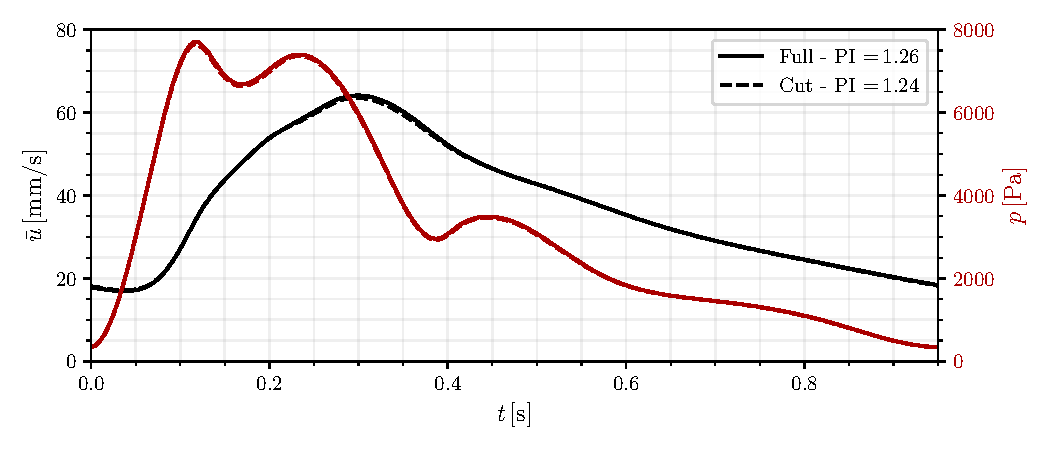
\includegraphics[width=\textwidth]{chapter5/Figures/Convergence/cut_full_comparison.pdf}
	\renewcommand{\arraystretch}{1.4}
	\setlength{\tabcolsep}{10pt}
	\begin{tabular}{cccccc}
		\toprule
		\multicolumn{2}{c}{\textbf{Comparison}} & \textbf{Mean}     & \textbf{Std} & \textbf{Min} & \textbf{Max}           \\
		\midrule
		\multirow{2}{*}{Full stent}             & $p\,$[\pa]        & 3257.65      & 2376.46      & 337.604      & 7708.38 \\
		                                        & $\bar{u}$\,[mm/s] & 37.5429      & 14.8827      & 16.9161      & 64.1167 \\
		\midrule
		\multirow{2}{*}{Cut stent}              & $p\,$[\pa]        & 3236.66      & 2361.91      & 333.288      & 7653.89 \\
		                                        & $\bar{u}$\,[mm/s] & 37.4279      & 14.7269      & 17.1103      & 63.5877 \\
		\bottomrule
	\end{tabular}
	\caption[Comparison between cut and full stents]{Comparison between the hemodynamics of using a full stent section and using a stent reduced to the areas exposed to neck and branches. The variables considered are the intra-aneurysmal velocity magnitude $\bar{u}$ (black), the pressure (red) and the Pulsatility Index (PI) given in the legend. These quantities are integrated over the aneurysm sack and normalized by the sack volume.}\label{fig:fullvscut}
\end{figure}

\begin{equation}
	\text{PI} = \frac{\max(\bar{u}) - \min(\bar{u})}{\text{mean}(\bar{u})}
\end{equation}


\section{Second Section}\label{chap5:sec2}

\section{Third Section}\label{chap5:sec3}

\bibliographystyle{elsarticle-num}
\bibliography{chapter5/Biblio}
% %%%%%%%%%%%%%%%%%%%%%%%%%%%%%%%%%%%%%%%%%%%%%%%%%%%%%%
\newpage
\pagestyle{fancy}

\chapter{Conclusions}\label{conclusion}
\minitoc
\newpage
\linenumbers
\section{Conclusion}
Decades of research in biomechanics have laid a foundation in clinical practice by developing virtual analysis tools for various cardiovascular diseases. These tools have not only enhanced our understanding of the origins of these pathologies but also facilitated the design of optimized treatment strategies. Building on this foundation, both this thesis and the ERC project CURE aim to improve diagnosis and treatment options for patients with intracranial aneurysms. This work focuses on three key research areas: (1) the study of stabilized finite elements for cardiovascular flows, (2) the assessment of the vascular extension around an aneurysm required for accurate numerical simulations, and (3) the development of a fast virtual stenting algorithm for deploying flow diverter stents. Although distinct, these aspects are united by a shared goal of advancing state-of-the-art modeling, with a strong emphasis on the numerical aspects of simulations.

In the second chapter, we delve into the physics and numerical methods for simulating hemodynamics in brain arterial flows. We revisited the existing numerical framework in a didactic manner, identifying an inconsistency in one modeling choice, which led to the research question: ``How can a tensor-based stabilization parameter become impervious to the ordering of elements?'' To address this, we developed a novel strategy based on Principal Component Analysis, testing it against common 2D and 3D examples from the literature. While not exhaustive, the validation showed improvements over an established alternative and consistently aligned well with experimental data.

With an improved understanding of the FEM backend, we explored the complex technical aspects of brain arterial flow, which is constrained by medical knowledge and limited measurement data. We reviewed the literature on boundary conditions and detailed the segmentation and meshing workflows implemented. This led to another research question: ``What is the extent of the vasculature that needs to be simulated around the region of interest to obtain physiological results, particularly when using common outflow models?'' This question arises from the segmentation of the anastomotic (redundantly connected) vessel network in the brain, where arterial loops can theoretically direct flow in any direction and do not always follow common splitting laws. We studied the sensitivity of three patient-specific cases with aneurysms, comparing full Circle of Willis simulations with two reduced vasculature models commonly seen in the literature. The results revealed case-dependent variability, suggesting the need for preliminary studies using different imaging sources to avoid modeling pitfalls.

The next focus was on flow diverter stents, which enable clinicians to treat otherwise inoperable intracranial aneurysms. A numerical representation of these devices not only replicates altered flow conditions but also provides insights into how hemodynamic changes affect vessel walls. We proposed a novel virtual stenting algorithm based on geometric analysis, validated it against literature cases, in-vitro experiments, and postoperative patient images. We then demonstrated how to embed the device into an arbitrary unstructured computational mesh and ran a test simulation. The proposed methodology offers three advantages: (i) accurate estimation of local stent porosities, (ii) robust and fast deployment, and (iii) reliance only on centerline information and manufacturer data for deployment. However, the method does not account for mechanical interactions with vessel walls and may underperform with significant stent undersizing.

Equipped with the essential tools for post-treatment aneurysm simulations, we examined three patient cases involving flow diverter stents with varying outcomes. The first case, featuring a giant aneurysm, suffered a delayed rupture after treatment. Simulations of preoperative and postoperative states including wall compliance were carried out and served an analysis based on several rupture hypotheses from the literature. The remaining cases involved (i) a ruptured blister aneurysm and (ii) a ruptured wide-necked aneurysm. Although different, both cases required assessing similar risks, including the trade-offs between reducing flow stress and managing thromboembolic complications. We report on the computed hemodynamics and include a study on deploying a second stent over the existing one. With these results, we hope to contribute to larger population studies aimed at optimizing treatment options.


\section{Perspectives}
The work is one of the two initial thesis conducted at the start of the aforementioned ERC project CURE\@. The project posed many initial hurdles thanks to which we learned and progressed. With the momentum gained, the subsequent work of other PhD students can tackle more specific problems. Among all the possible modalities to follow, there are some that are of particular interest in the context of flow diverters.

Firstly, thrombosis has been observed in literature and in one of the presented cases, to lead in some cases to wall autolysis and aneurysm rupture. Simulating thrombosis can help confirming or disproving the autolysis hypothesis by provding the growth dynamics and the exposure time of damaged tissue. Furthermore, it could also be applied to optimize stent design in order to achieve an optimal occlusion rate. The latter optimization has already been conducted by the team, exploiting the capabilities of Reinforcement Learning, but using a reduced simulation complexity\,\cite{Hachem2023}. These ideas can be pursued with more elaborate modelling techniques for which parts of the study will serve. The porosity maps from the stenting algorithm can be used in combination with novel continuum models\,\cite{Abdehkakha2021} of flow diverters to yield a light-weight, yet accurate method for optimization purposes. The Reinforcement Learning has also been advanced in our team ever since\,\cite{Hachem2023} thanks to an improved environment based on partial differential equations\,\cite{Viquerat2024}. With these tools it may become part of clinical routine to design and process personalized medical devices that adjust to each patient's needs at feasible cost.

Validation to this ambitious goal is more increasingly available thanks to improved fields strengths and frame rates of Magnetic Resonance and Computed Tomography machines. With the help of Machine Learning in denoising and gap-filling measurements, the adquisition of reliable data could be carried out as part of clinical routine. This in turn helps validating new algorithms and tackles at the same time the limitiations imposed by using generic boundary conditions. 

\nolinenumbers

\bibliographystyle{apsrev}
{\footnotesize
	\bibliography{chapter5/Biblio}}

%\appendix
%\chapter{First Appendix} \label{appendix:ap2}

\end{document}
